\documentclass[a4paper,11pt]{article}
\usepackage{graphicx}
\usepackage{url}
\usepackage{amsmath}
\usepackage{amsfonts}
\usepackage{geometry}
\usepackage[numbers]{natbib}
\usepackage{cite}
\usepackage{listings}
\usepackage{hyperref}
\geometry{margin=1in}
\bibliographystyle{plain}
\graphicspath{{../../04-outputs/03-spotify-valence-replication/}}

\title{Replication Study: Valence Prediction and Trend Analysis in Spotify Audio Features}
\author{}
\date{}

\begin{document}

\maketitle

\section*{Abstract}
This replication study revisits the findings of Dutta and Mookherjee (2023) \citep{dutta2023emotional}, who investigated the emotional character of music using valence scores from Spotify audio features. We use a more extensive dataset comprising over 160,000 tracks recorded between 1921 and 2020 to reproduce and extend their analysis. Through exploratory data analysis, we examine how valence varies over time and in relation to features like danceability, energy, and acousticness. Our visualizations reinforce their findings and reveal additional insights into the structure of musical emotion in modern streaming data.

\section{Introduction}
Streaming platforms like Spotify have made large-scale musical datasets widely accessible, allowing for detailed statistical analysis of audio features. One of the most meaningful among these is \textit{valence}, which represents the positivity or happiness conveyed by a track. A valence score of 0 denotes emotionally negative content (e.g., sad, angry), while a score of 1 indicates high emotional positivity (e.g., joyful, euphoric).

Building on the original work by Dutta and Mookherjee (2023) \citep{dutta2023emotional}, this study examines how valence has evolved over the last century and how it correlates with other musical features. We replicate several of their visual analyses, aiming to validate their conclusions and provide a broader empirical foundation using a larger dataset. We begin with exploratory data analysis (EDA), the basis for understanding any downstream modeling or inference.

\section{Exploratory Data Analysis (EDA)}

\subsection{Data Preprocessing}
The \href{https://www.kaggle.com/datasets/yamaerenay/spotify-dataset-1921-2020-160k-tracks}{original dataset}, sourced from Spotify via Kaggle, contained over 160,000 tracks spanning the years 1921 to 2020. To maintain computational efficiency while preserving representativeness, we randomly sampled 10,000 tracks from this dataset using a fixed seed to ensure reproducibility.

During preprocessing, we removed redundant columns unrelated to the modeling objectives, such as track names, artist lists, popularity scores, and identifiers. We also excluded rows with missing values in key audio features and converted relevant columns to appropriate types (e.g., \texttt{year} as integer, \texttt{key} and \texttt{mode} as factors). These steps ensured a clean, consistent dataset for analysis.

\subsection{Valence Distribution}
We begin with an overview of the emotional landscape by examining the distribution of valence scores (Figure~\ref{fig:valence_distribution}). The distribution appears broadly uniform across the range [0, 1], with a modest concentration around 0.5-0.6. This suggests that many songs tend to fall into the moderately positive emotional range. Tracks with extreme valence scores\textemdash either highly negative or highly positive\textemdash are less common, potentially reflecting listener preferences or production tendencies that favor more emotionally balanced content.

\begin{figure}[h]
\centering
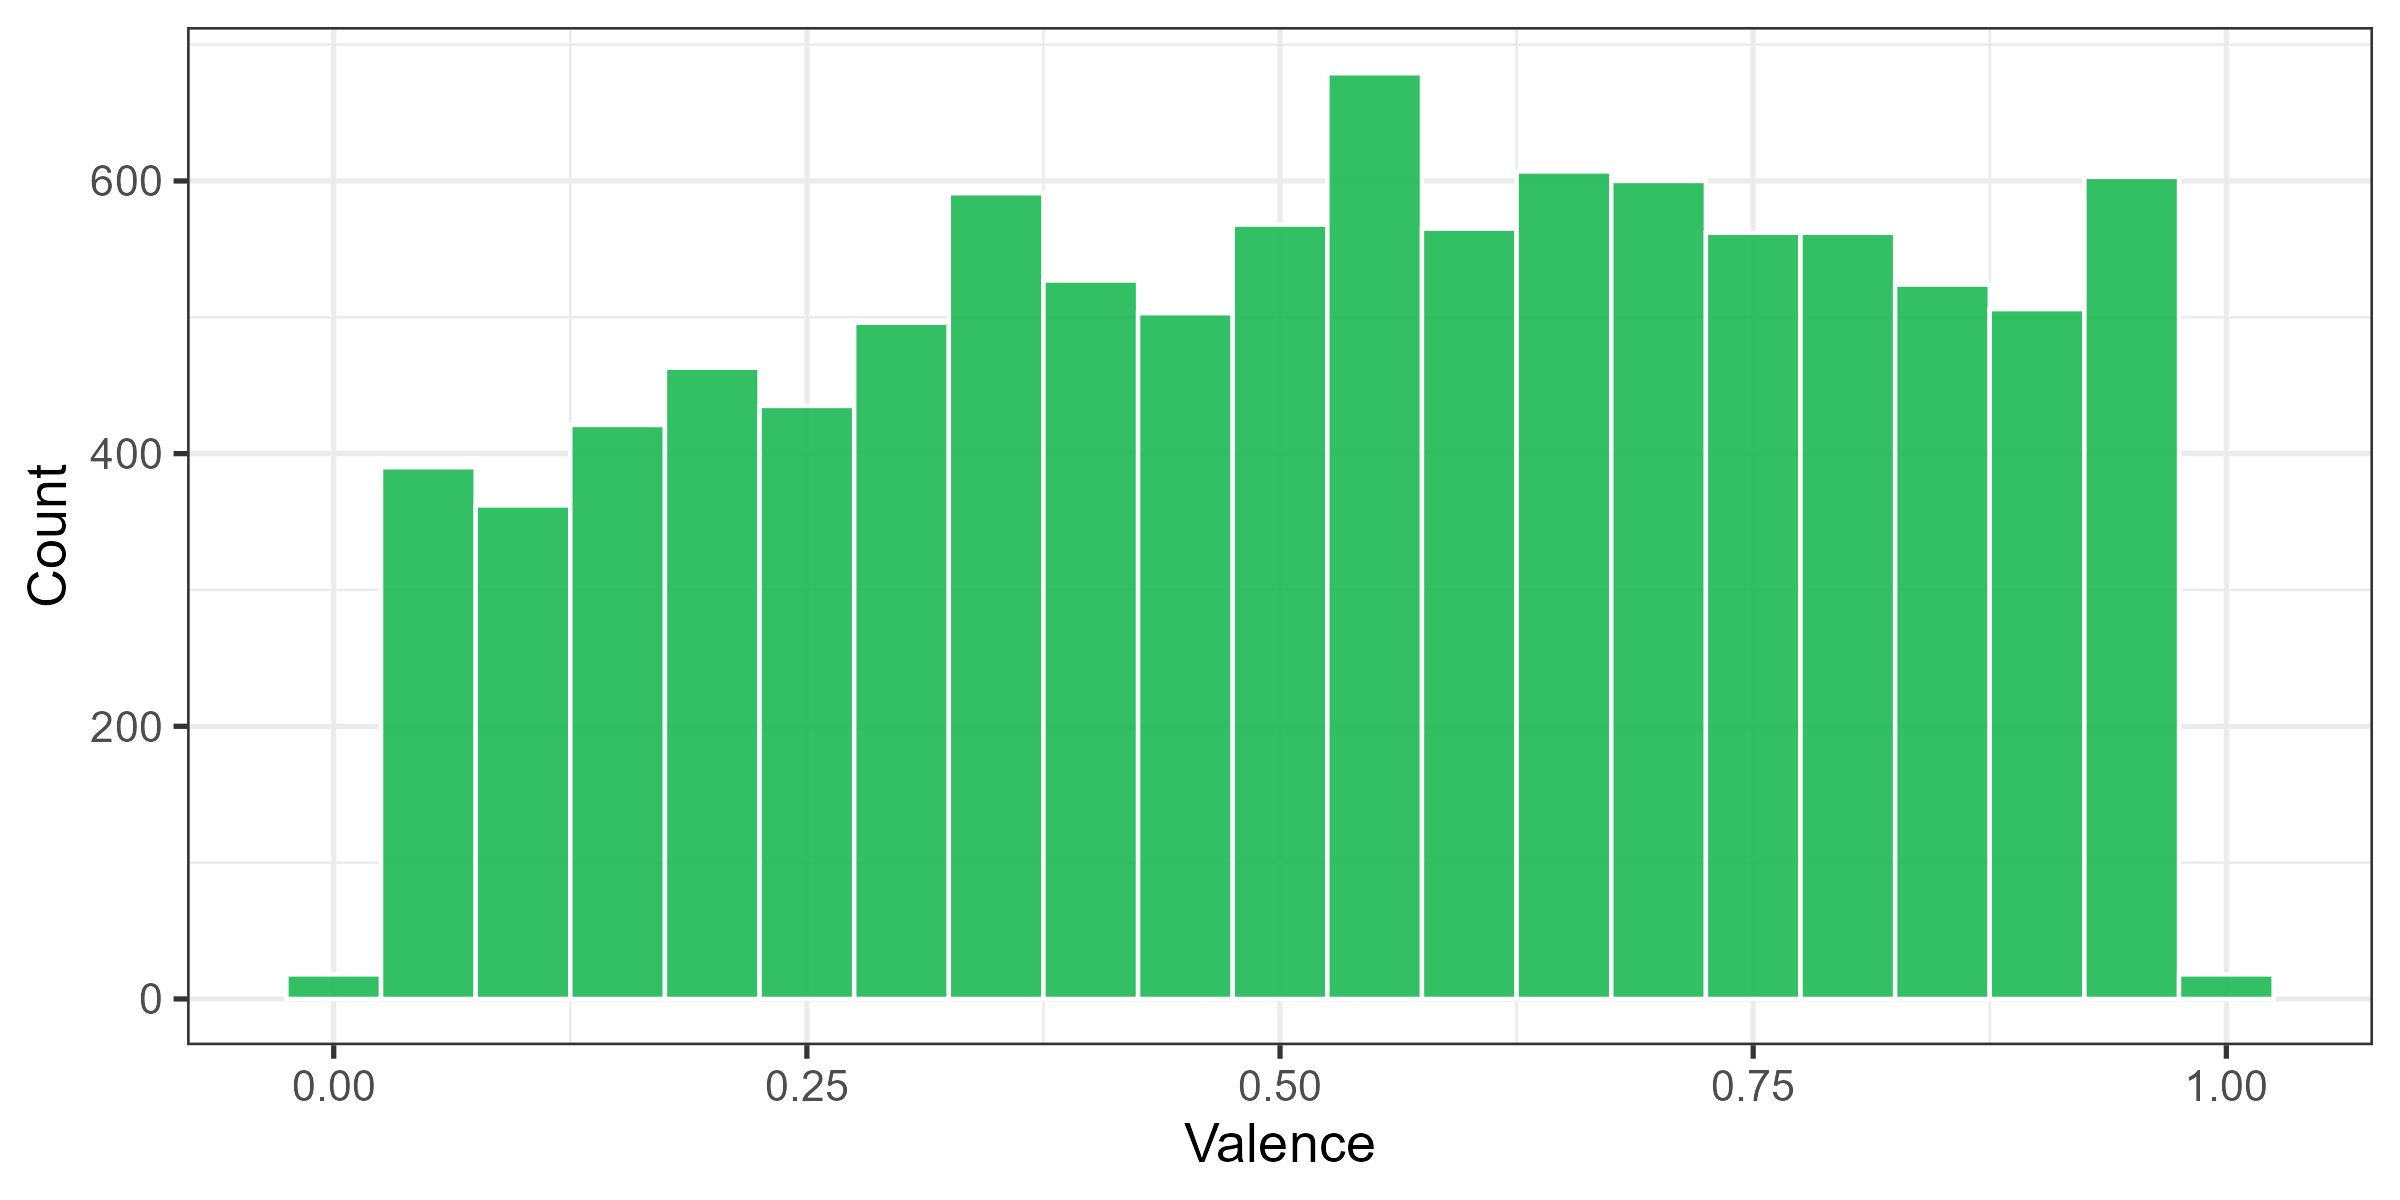
\includegraphics[width=0.85\textwidth]{Figure1-valence-distribution.png}
\caption{Distribution of valence scores across Spotify tracks from 1921 to 2020. A moderate central peak suggests a slight preference for emotionally neutral or mildly positive music.}
\label{fig:valence_distribution}
\end{figure}

\subsection{Temporal Evolution of Valence}
To explore how the emotional tone of music has changed over time, we computed the average valence score per year and plotted the results in Figure~\ref{fig:valence_trend}. A clear trend emerges: while valence values fluctuated across decades, there is a noticeable downward drift starting in the 1980s. This may indicate that popular music has become, on average, less upbeat or emotionally bright in recent decades. Notably, the period between 1950 and 1975 shows relative emotional stability in musical output.

\begin{figure}[h]
\centering
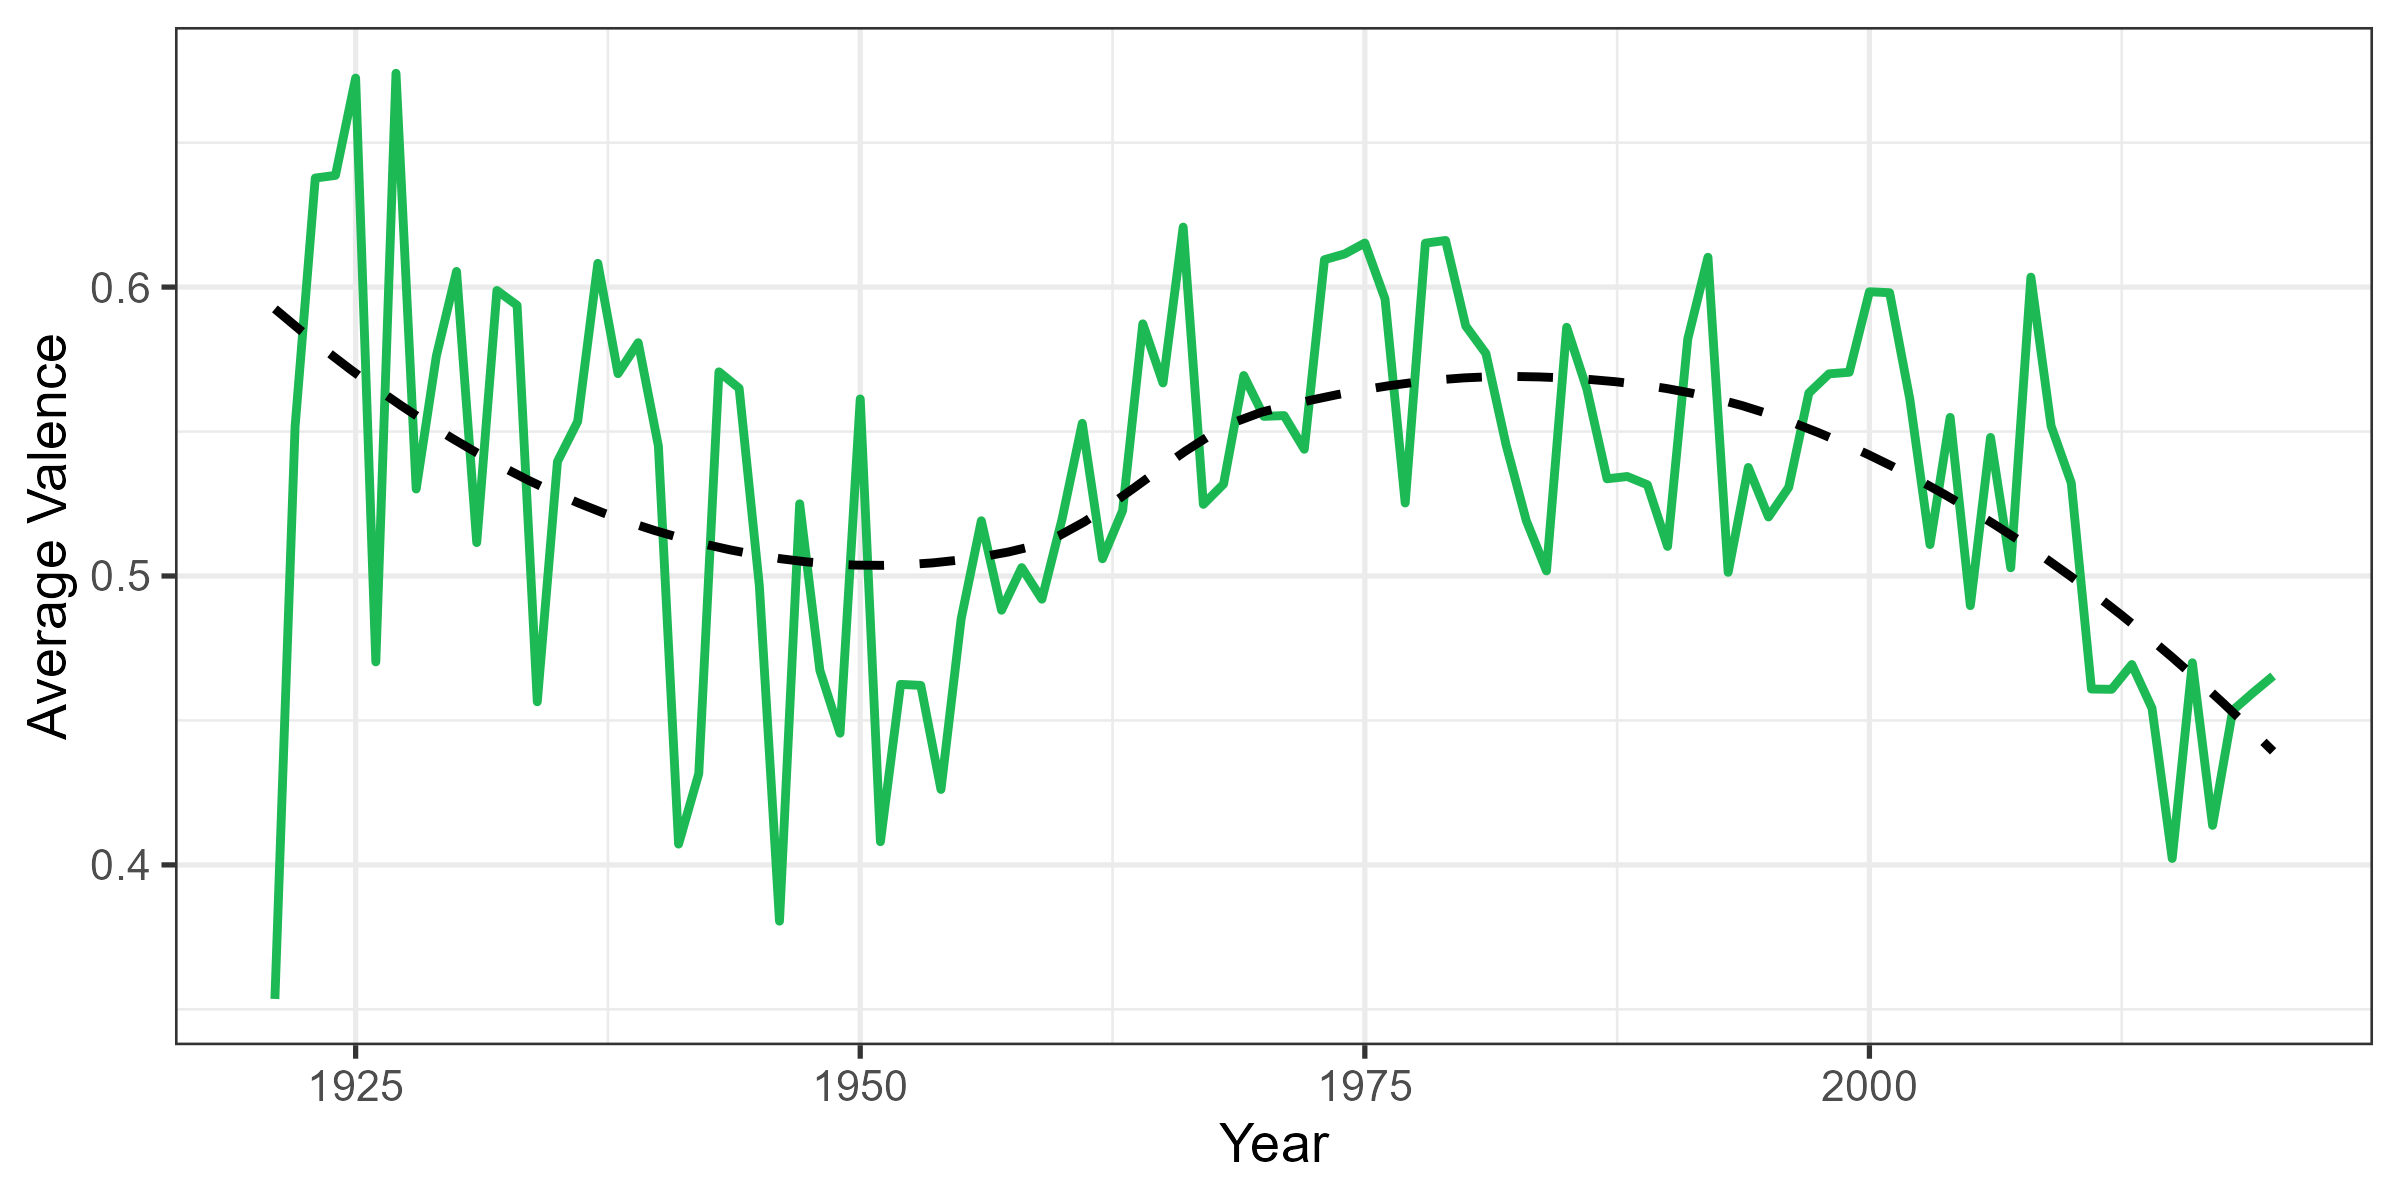
\includegraphics[width=0.85\textwidth]{Figure2-valence-trend-year.png}
\caption{Average valence per year from 1921–2020. A loess curve reveals a gradual long-term decline in musical positivity.}
\label{fig:valence_trend}
\end{figure}

\subsection{Danceability and Valence}
In Figure~\ref{fig:scatter_dance}, we visualize the relationship between valence and danceability. A positive association is apparent: as danceability increases, valence also tends to rise. This aligns with intuition, as tracks designed for dancing are often rhythmically engaging and emotionally uplifting. That said, the scatterplot shows considerable spread, especially in the mid-valence range, indicating that danceability alone is not a strong predictor of emotional tone.

\begin{figure}[h]
\centering
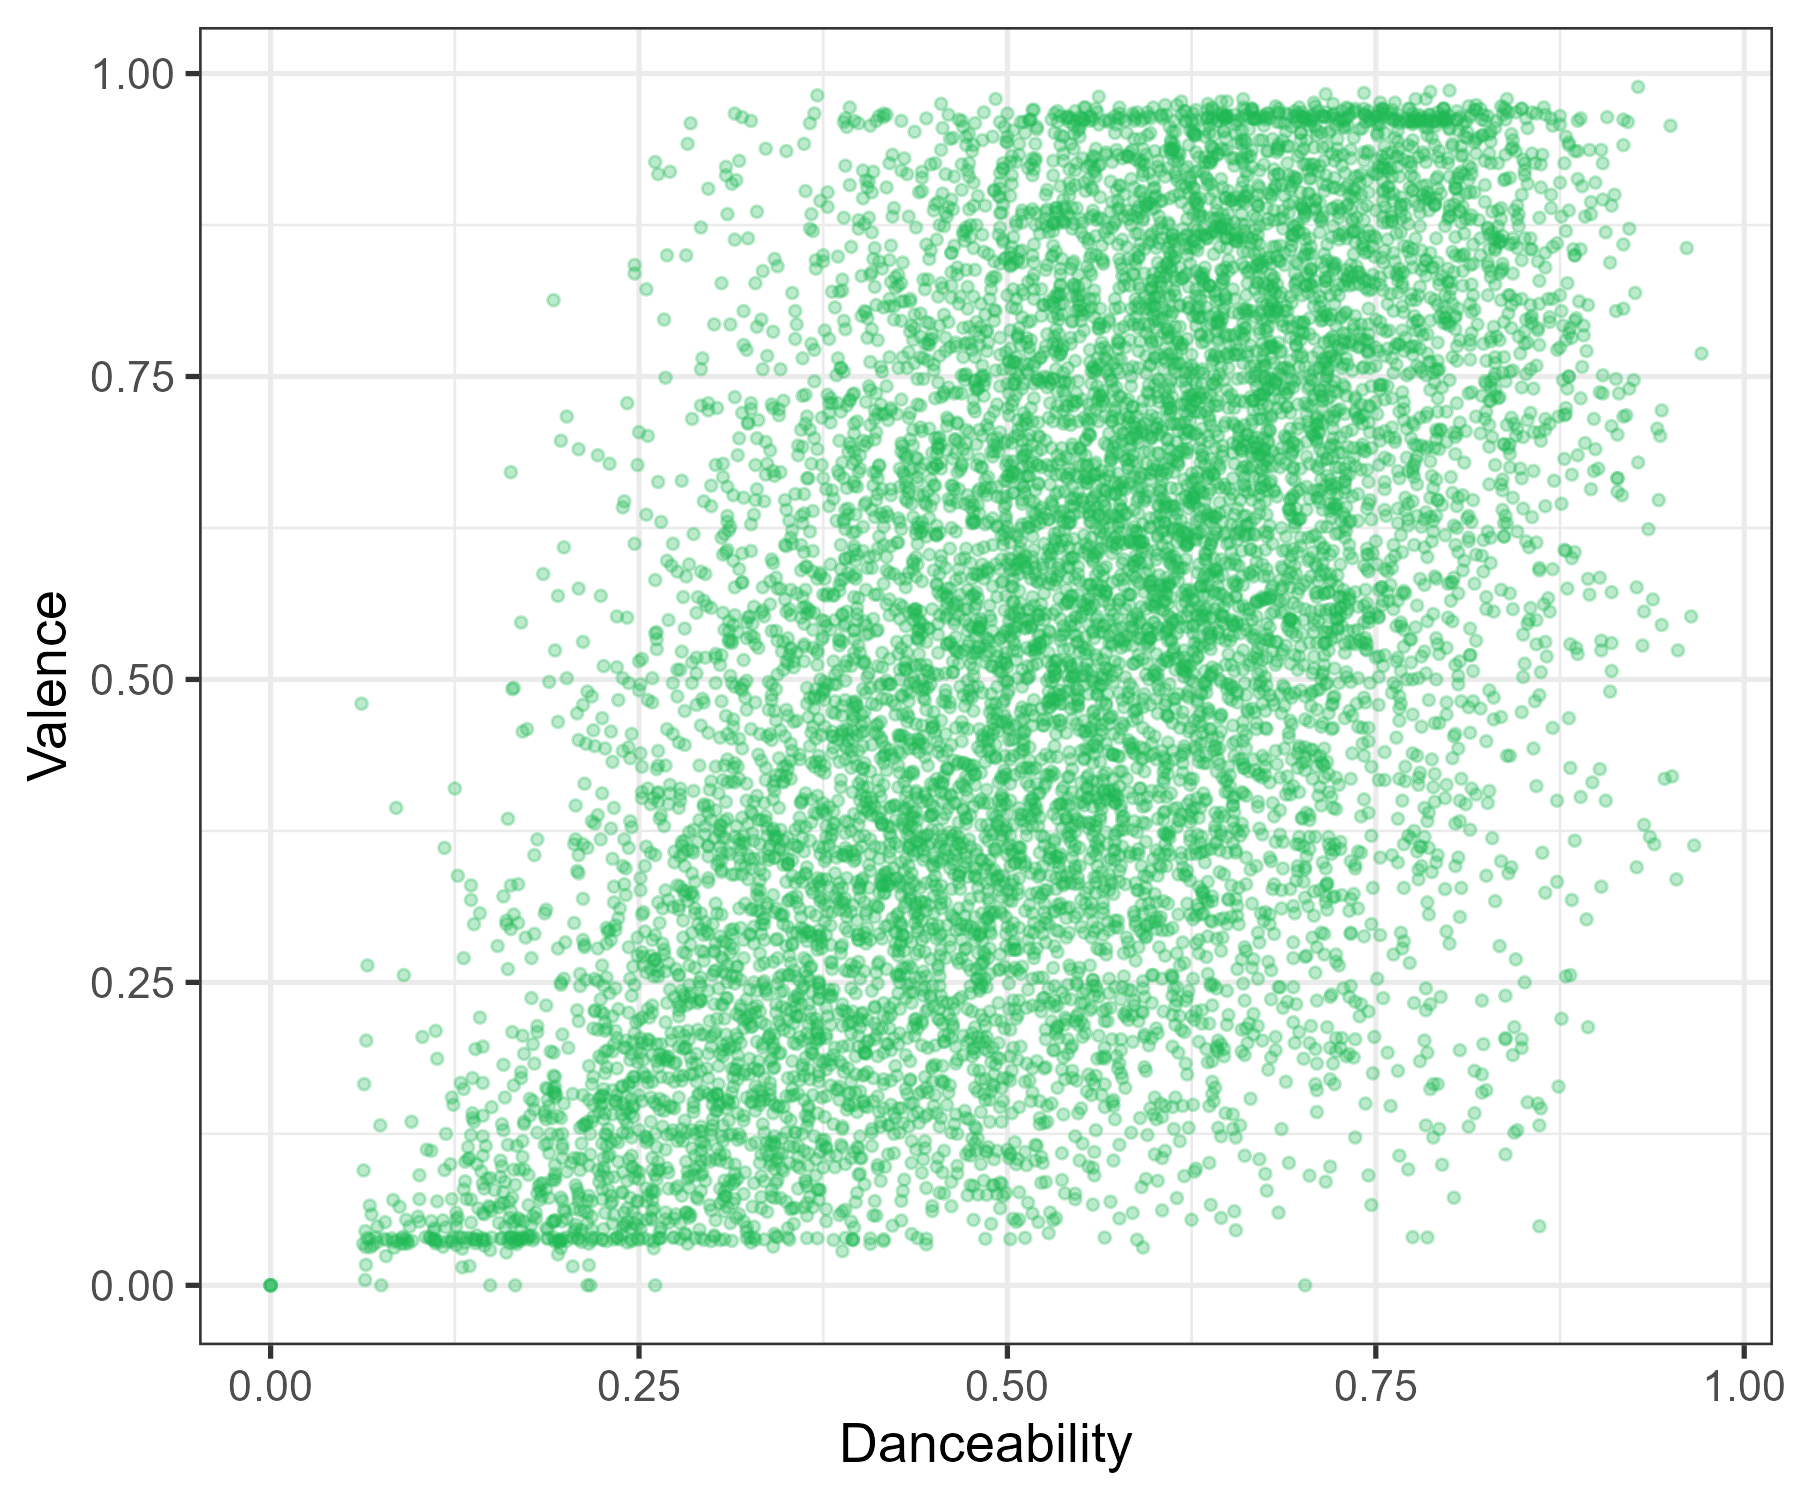
\includegraphics[width=0.75\textwidth]{Figure3-scatter-danceability-valence.png}
\caption{Scatter plot of valence vs danceability. While the relationship is noisy, a loose positive association is visible.}
\label{fig:scatter_dance}
\end{figure}

\subsection{Pairwise Feature Relationships}
To explore inter-feature relationships more broadly, we created a pair plot of valence, energy, acousticness, and danceability (Figure~\ref{fig:pairplot}). The plot highlights a strong positive relationship between valence and both energy and danceability, suggesting that more energetic and rhythmically appealing songs tend to be perceived as happier. In contrast, acousticness exhibits a slight negative correlation with valence, consistent with the idea that acoustic tracks are more introspective or somber.

\begin{figure}[h]
\centering
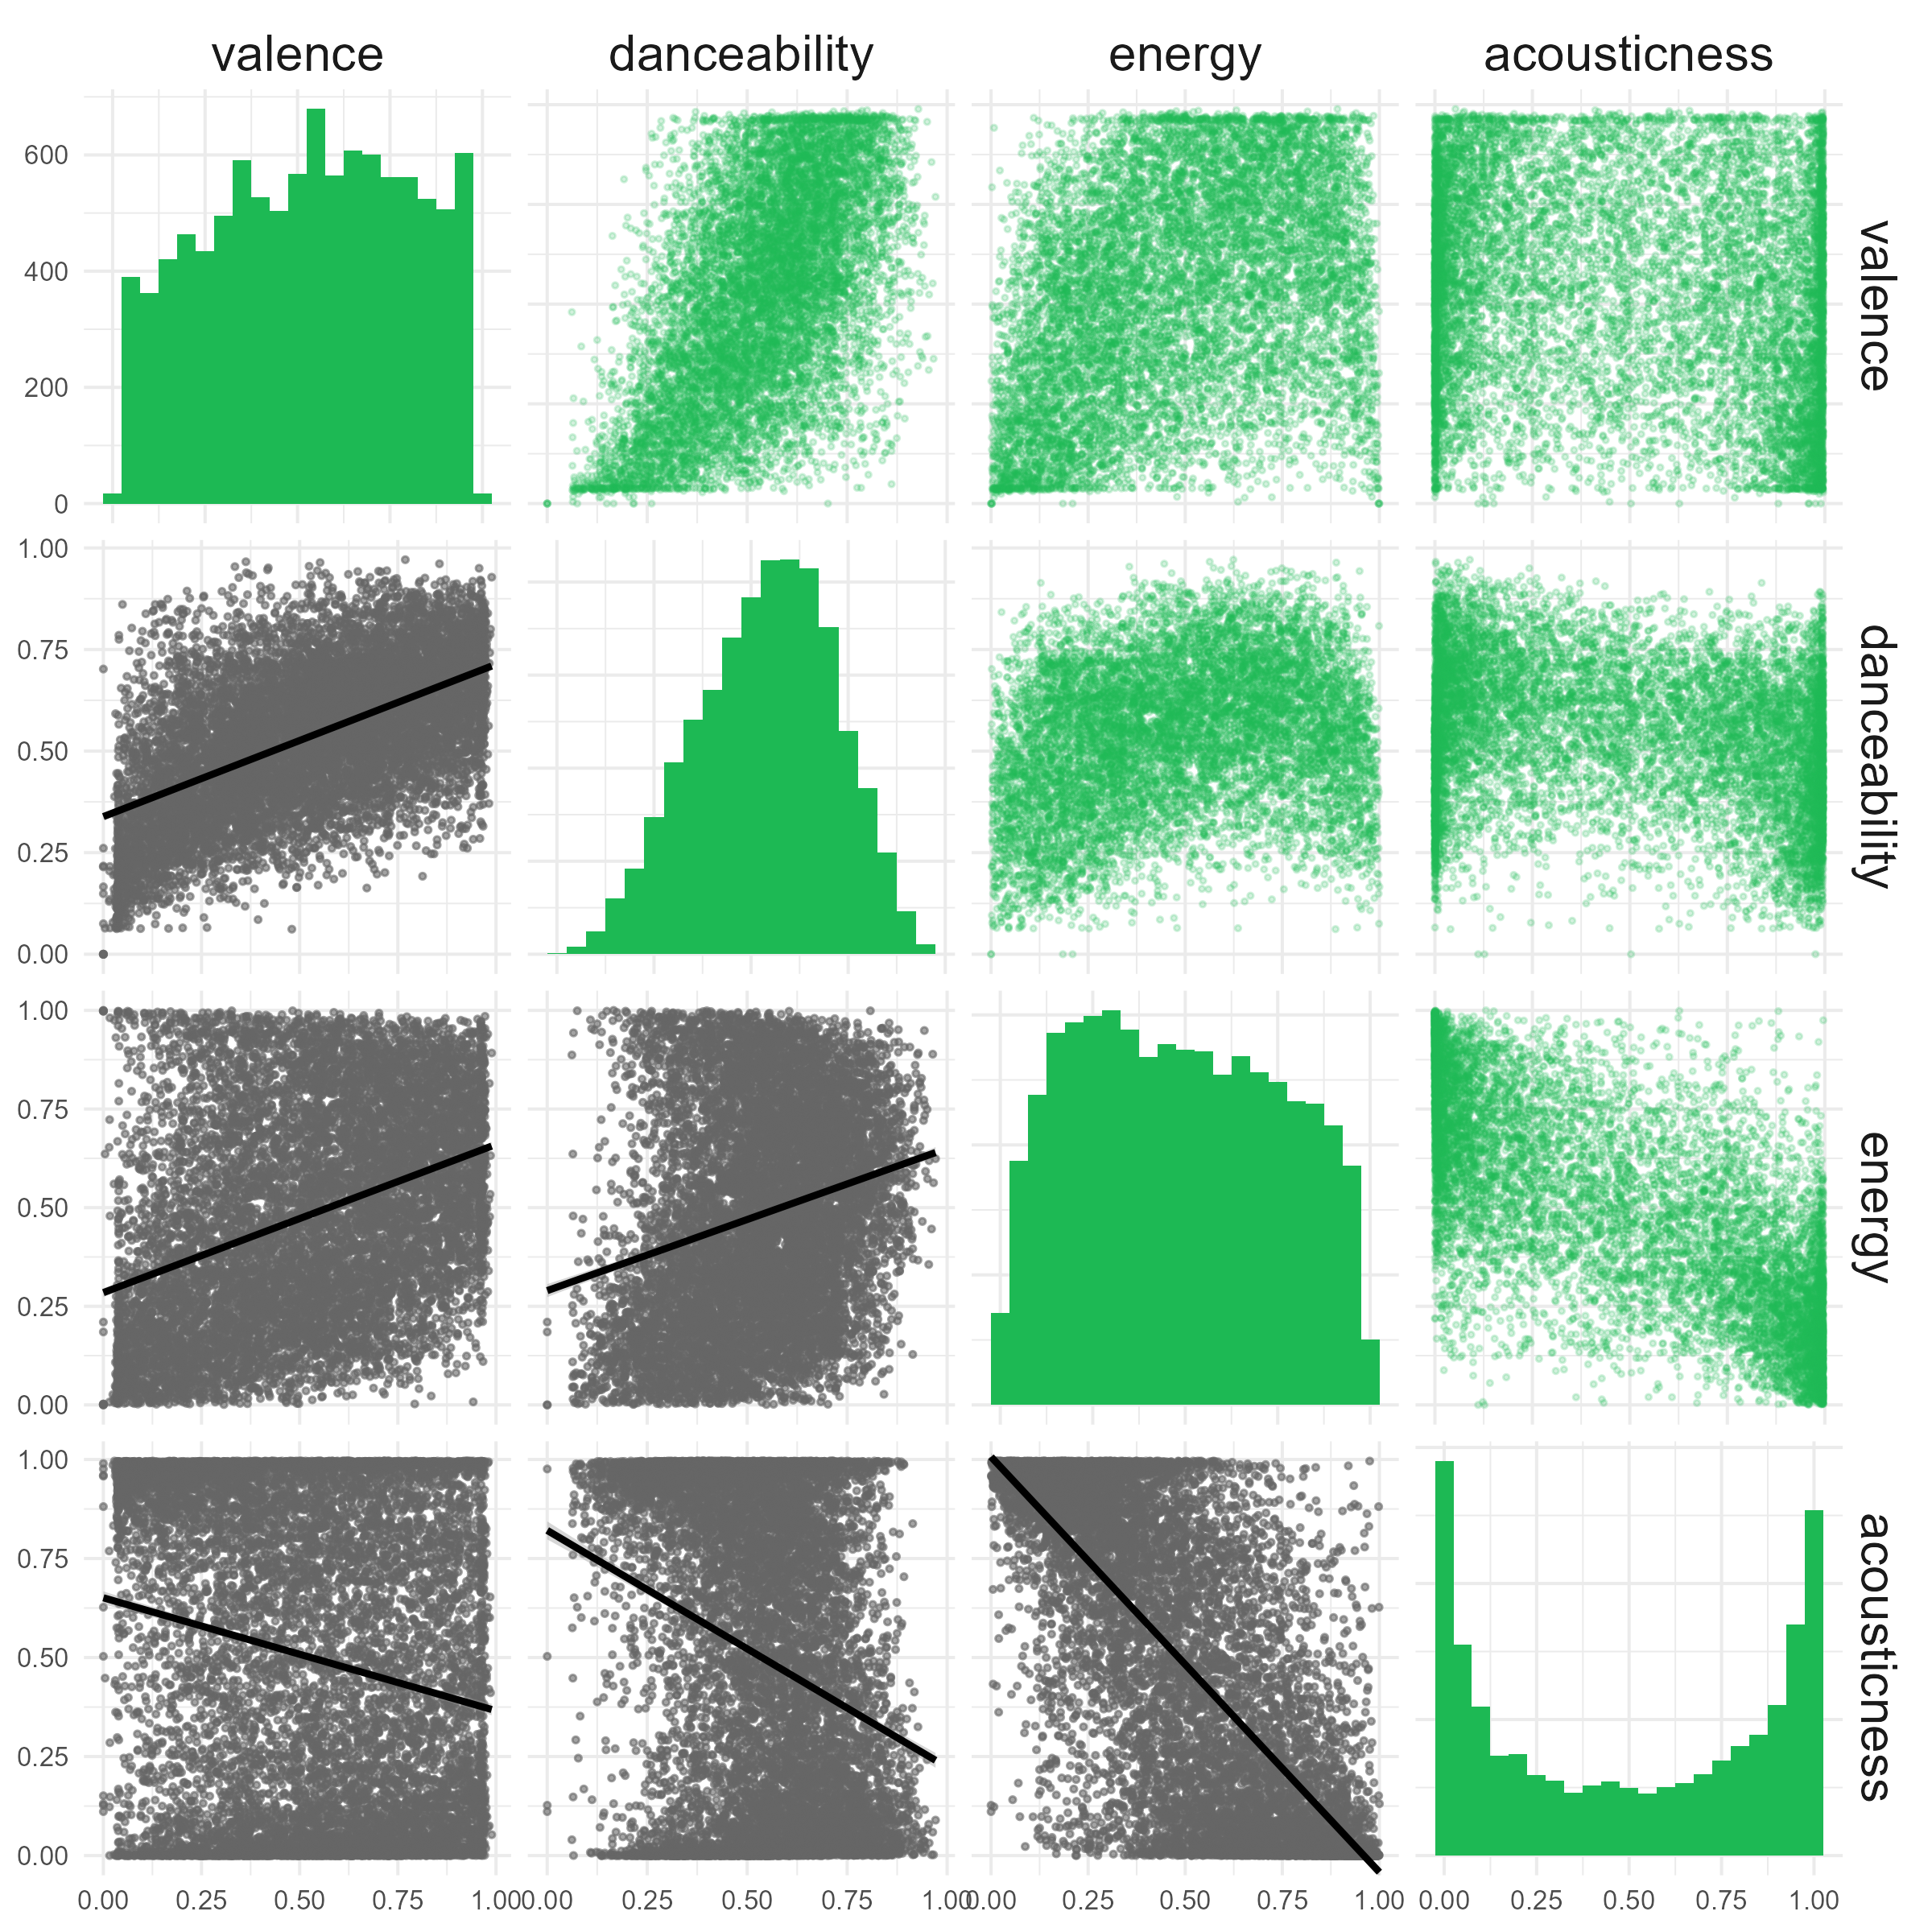
\includegraphics[width=0.65\textwidth]{Figure4-pairplot-valence.png}
\caption{Pairwise plots among valence, danceability, energy, and acousticness. Positive relationships are observed between valence and both energy and danceability.}
\label{fig:pairplot}
\end{figure}

\subsection{Correlation Heatmap of Features}
Finally, we examined the pairwise correlations between key audio features used in valence prediction (Figure~\ref{fig:corr_matrix}). Valence correlates positively with both danceability and energy, and negatively with acousticness\textemdash supporting trends seen in earlier plots. Other strong correlations include a tight link between energy and loudness (positive), and a negative association between acousticness and loudness. These findings confirm that emotional tone in music is influenced by overlapping dimensions of audio features.


\begin{figure}[h!]
\centering
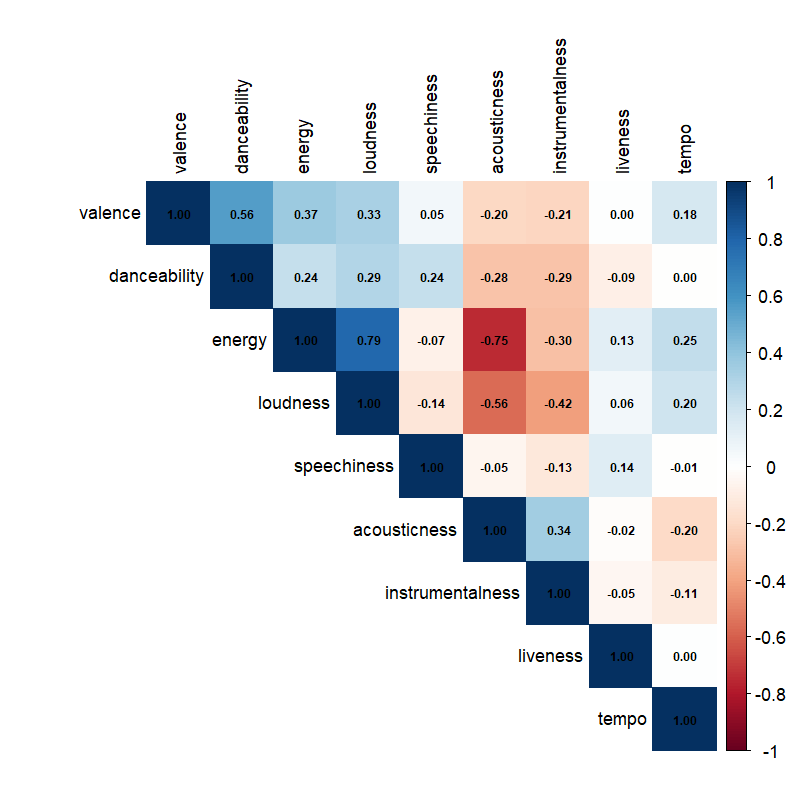
\includegraphics[width=0.65\textwidth]{Figure5-correlation-matrix.png}
\caption{Correlation matrix among Spotify audio features. Valence is positively associated with danceability and energy, and negatively associated with acousticness.}
\label{fig:corr_matrix}
\end{figure}

\section{Modeling and Results}

\subsection{Regression Modeling}
To investigate which audio features most strongly influence perceived emotional tone in music, we constructed two predictive models: linear regression and random forest. Both models were trained on a stratified random sample of 70\% of the dataset, with the remaining 30\% reserved for testing. The objective was to estimate the valence score\textemdash Spotify’s proxy for musical happiness\textemdash based on a set of numerical and categorical audio descriptors.

The linear regression model provides a useful interpretative baseline, allowing us to assess the direction and magnitude of feature contributions under a linear assumption. In contrast, the random forest model is a non-parametric ensemble method that captures complex interactions and non-linearities. This dual approach gives us a clearer view of which features matter, and how.

\subsection{Model Evaluation}
We evaluated model performance using four common metrics: mean absolute error (MAE), mean squared error (MSE), root mean squared error (RMSE), and the coefficient of determination ($R^2$). Table~\ref{tab:model_performance} reports these results.

\begin{table}[h]
\centering
\begin{tabular}{lcccc}
\hline
\textbf{Model} & \textbf{MAE} & \textbf{MSE} & \textbf{RMSE} & \textbf{$R^2$} \\
\hline
Linear Regression & 0.1546 & 0.0362 & 0.1902 & 0.3691 \\
Random Forest     & 0.1487 & 0.0341 & 0.1847 & 0.3924 \\
\hline
\end{tabular}
\caption{Performance of each model on the test data (30\% split).}
\label{tab:model_performance}
\end{table}

The random forest model outperformed linear regression across all metrics, though the improvements were modest. This suggests that while linear relationships explain some variance in valence, non-linear patterns and feature interactions add incremental predictive value.

\subsection{Feature Importance}
The random forest model also offers a convenient mechanism for evaluating the relative contribution of each input variable through permutation-based importance metrics. Figure~\ref{fig:feature_importance} ranks the top predictors of valence according to their impact on model error.

\begin{figure}[h]
\centering
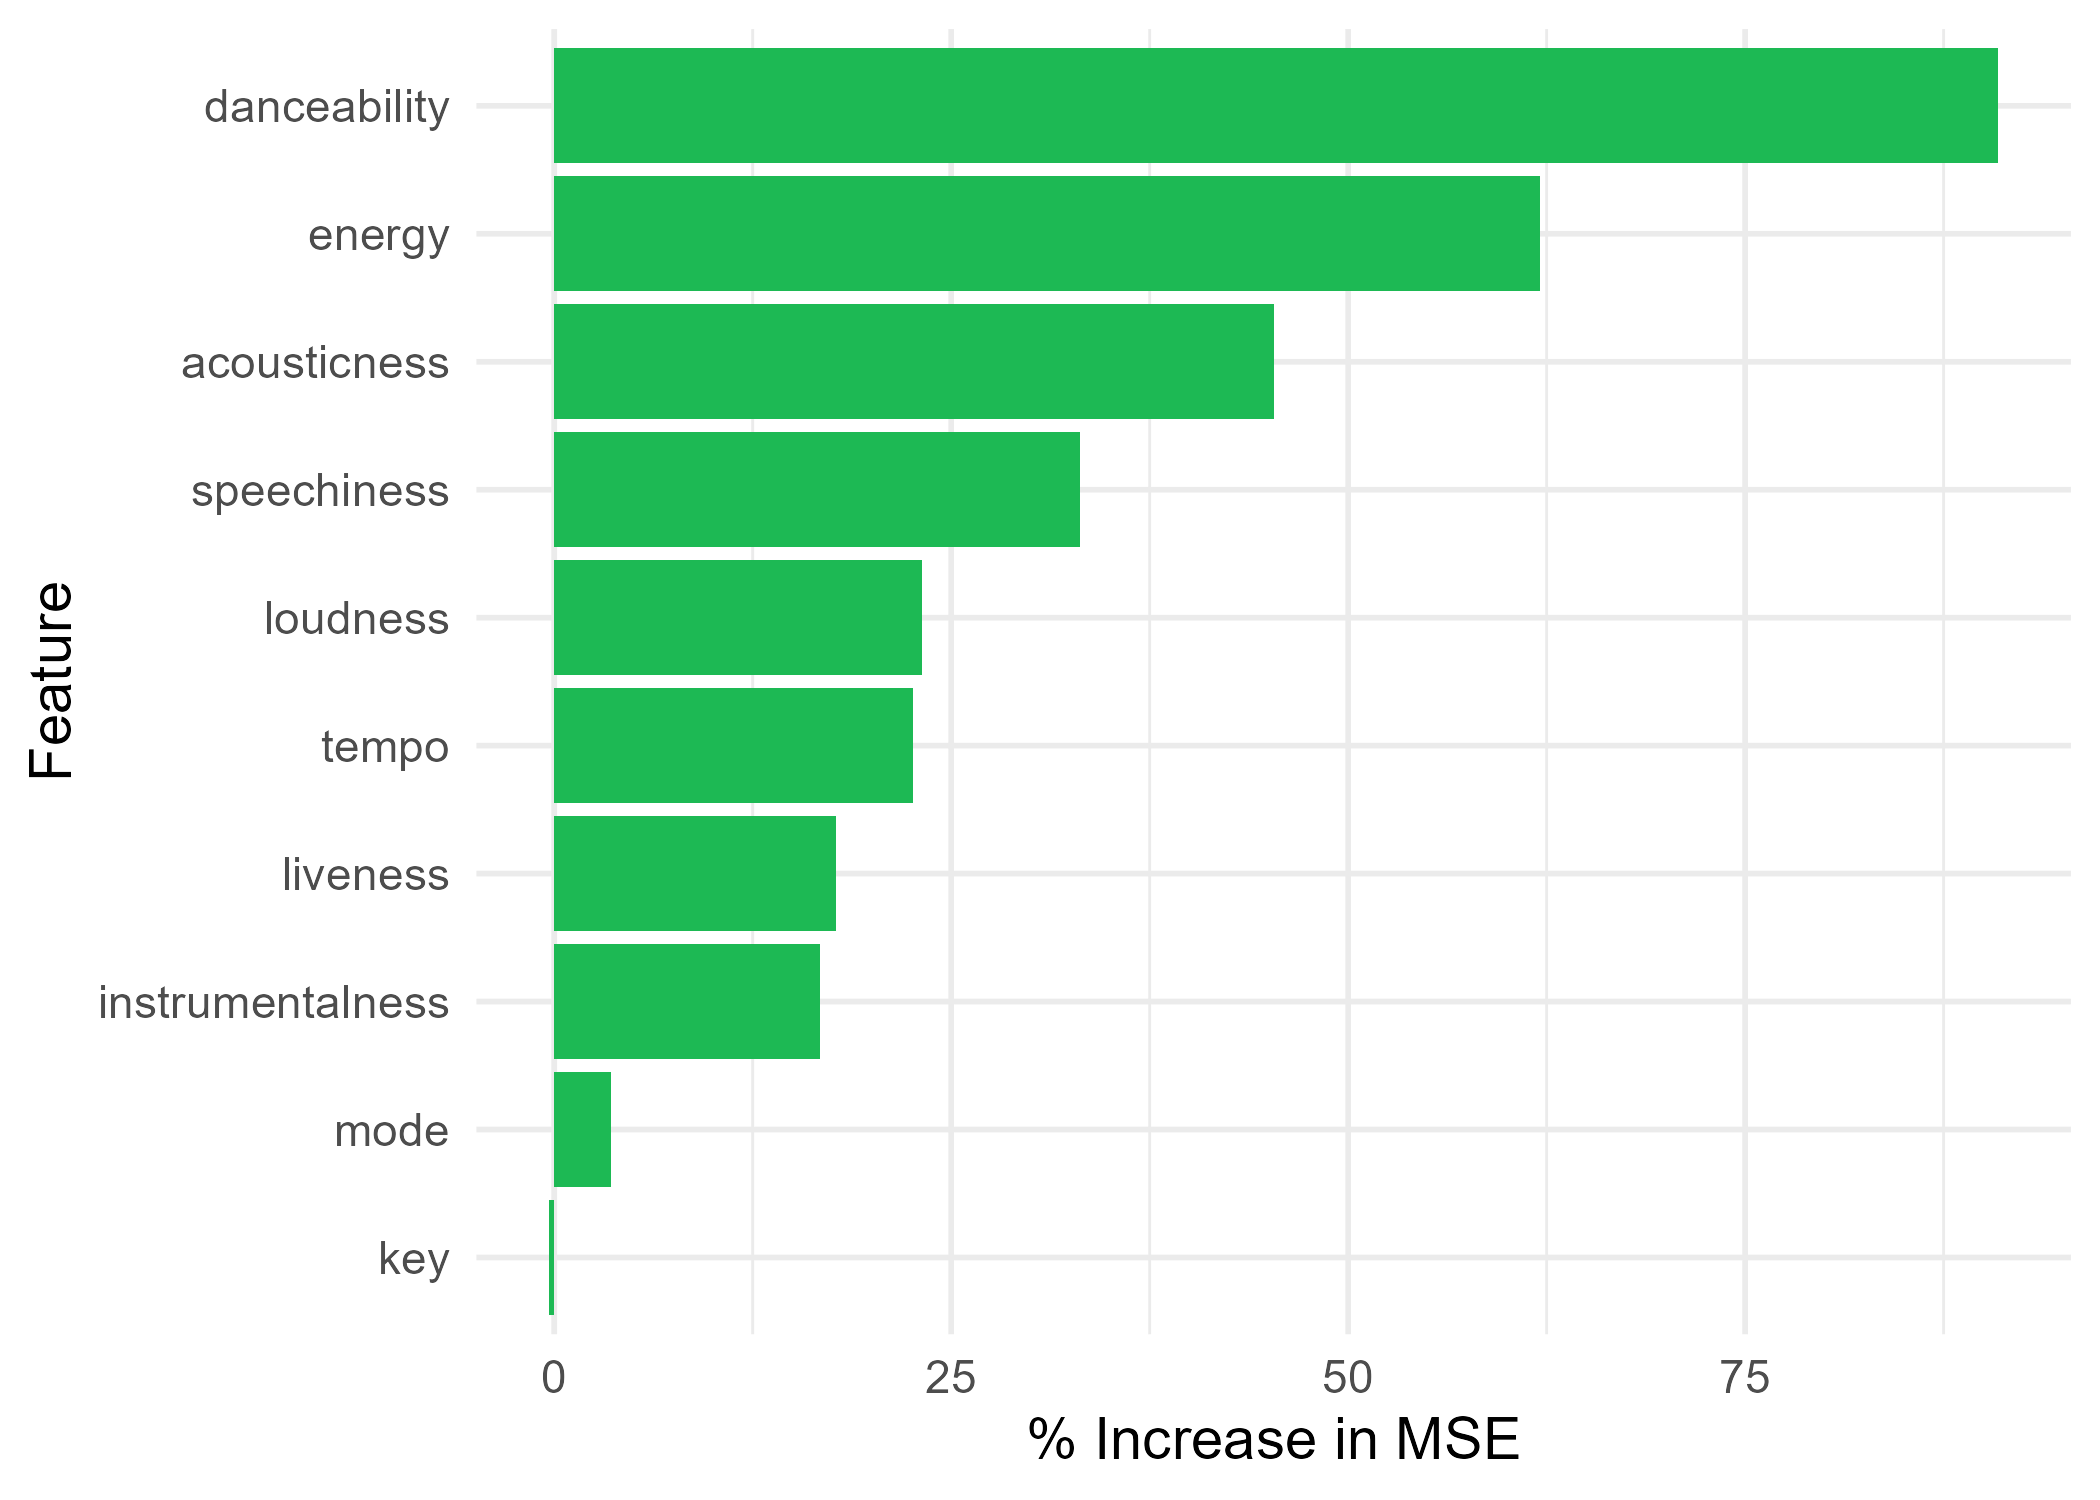
\includegraphics[width=0.85\textwidth]{Figure6-rf-feature-importance.png}
\caption{Random forest feature importance scores, measured by percent increase in MSE when each feature is permuted.}
\label{fig:feature_importance}
\end{figure}

As expected, \texttt{danceability} emerged as the most influential feature, suggesting that rhythm and movement are strong indicators of musical positivity. \texttt{Energy} also ranked highly, consistent with the idea that faster and more intense songs tend to sound happier. Features such as \texttt{acousticness} and \texttt{speechiness} contributed moderately, while categorical features like \texttt{key} and \texttt{mode} had minimal influence.

\section{Conclusion}
This study replicated and extended the findings of Dutta and Mookherjee (2023), using a larger and more recent Spotify dataset to investigate the emotional character of music. We reproduced key exploratory analyses and built predictive models that confirmed the relevance of features like danceability and energy for estimating valence.

Our results reinforce several intuitive ideas: happy-sounding songs are typically more danceable and energetic, while quieter or acoustically sparse tracks lean toward somberness. Additionally, our models showed that even relatively simple features can explain a significant portion of valence variability, though not all of it. This suggests that valence, while quantifiable, also depends on subtleties not easily captured by numerical descriptors alone.

Future extensions might involve genre-specific modeling, temporal forecasting of mood trends, or incorporating listener-level data to personalize emotion predictions. These directions offer exciting opportunities for music informatics and computational creativity.

\bibliography{bibliography}

\end{document}